\documentclass[10pt,twocolumn]{article}

% --- geometry and basic typography ---
\usepackage[a4paper,margin=0.85in,columnsep=0.25in]{geometry}
\usepackage[T1]{fontenc}
\usepackage{lmodern}
\usepackage{microtype}

% --- math and graphics ---
\usepackage{amsmath,amssymb}
\usepackage{graphicx}
\graphicspath{{../}{../figures/}{figures/}}

% --- tables and floats ---
\usepackage{booktabs}
\usepackage{array}
\renewcommand{\arraystretch}{1.10}
\usepackage[skip=4pt]{caption}
\usepackage[section]{placeins}
\usepackage{flushend}

% --- algorithms ---
\usepackage{algorithm}
\usepackage{algpseudocode}

% --- references ---
\usepackage[numbers,sort&compress]{natbib}
\usepackage{hyperref}
\usepackage{url}

% --- author block ---
\usepackage{authblk}

% --- whitespace around floats: tight, no dead space ---
\setlength{\intextsep}{5pt plus 1pt minus 1pt}
\setlength{\textfloatsep}{6pt plus 1pt minus 1pt}
\setlength{\floatsep}{6pt plus 1pt minus 1pt}
\setlength{\dbltextfloatsep}{6pt plus 1pt minus 1pt}
\setlength{\dblfloatsep}{6pt plus 1pt minus 1pt}
\setlength{\abovecaptionskip}{3pt}
\setlength{\belowcaptionskip}{2pt}

% --- boundary-overflow safety valves ---
\emergencystretch=2em
\tolerance=2000
\hyphenpenalty=50
\sloppy

% --- house-style helpers ---
\newcommand{\best}[1]{\textbf{#1}}

\title{Transfer Learning on CIFAR-10: A Controlled Comparison of ImageNet-Pretrained Backbones}
\author[1]{Vikash Chandra Mishra\\\texttt{crimsonsyrus000@gmail.com}}
\affil[1]{Independent Researcher}
\date{}

\begin{document}
\twocolumn[
\maketitle
\begin{@twocolumnfalse}
\begin{abstract}
Training accurate image classifiers from scratch on small datasets such as CIFAR-10 typically demands long schedules and aggressive regularization, and even then often falls short of what large pretrained backbones can deliver out of the box. We study how much of that gap can be closed by simple ImageNet transfer learning under a tight twenty-epoch budget. Concretely, we replace the classifier heads of three standard ImageNet-pretrained backbones, VGG-16, MobileNetV2, and ResNet-18, and fine-tune the last residual block at a lower learning rate while training the head at a higher rate, using AdamW, batch size 128, light augmentation, and early stopping. Across three random seeds per model, ResNet-18 attains \textbf{91.5 $\pm$ 0.3}\% test accuracy on CIFAR-10, an absolute improvement of $13.6$ percentage points over a small from-scratch convolutional baseline ($77.9 \pm 0.7$\%). MobileNetV2 reaches $89.8 \pm 0.4$\% with substantially fewer parameters, offering the best accuracy-efficiency trade-off, and VGG-16 reaches $88.7 \pm 0.5$\%. Ablations show that unfreezing the final residual block contributes $4.3$ points and standard augmentation contributes $2.6$ points, and that pretrained models exceed $85$\% validation accuracy within five epochs while the from-scratch baseline has not converged by epoch twenty. The findings provide a clean, reproducible reference point for transfer-learning practice on small image-classification benchmarks.
\end{abstract}
\vspace{0.6em}
\end{@twocolumnfalse}
]

\section{Introduction}
Image classification is one of the most heavily studied problems in computer vision, and CIFAR-10~\cite{krizhevsky2009cifar} remains a workhorse benchmark for prototyping new ideas, comparing architectures, and teaching deep learning. Despite its small size (60{,}000 colour images, 32 by 32 pixels, ten balanced classes), it preserves enough visual variety to surface most of the design choices that matter on larger datasets: feature reuse across classes, sensitivity to data augmentation, the trade-off between model capacity and overfitting, and the cost of training a deep network from random weights. A natural question, particularly for practitioners with limited compute, is how much of the heavy lifting on CIFAR-10 can be offloaded onto features already learned at scale on ImageNet~\cite{deng2009imagenet}, and which design choices in the transfer pipeline actually carry the gain.

Three observations motivate the present study. First, modern ImageNet-pretrained backbones such as ResNet~\cite{he2016resnet}, VGG~\cite{simonyan2014vgg}, and MobileNetV2~\cite{sandler2018mobilenetv2} are now small and cheap enough to fine-tune on a single commodity GPU, yet practitioners new to the area often default to training a custom convolutional network from scratch and accept whatever accuracy the optimizer produces. Second, prior comparisons of these backbones on CIFAR-10 are scattered across blog posts, tutorials, and individual papers that use different optimizers, schedules, augmentations, and evaluation protocols, which makes it hard to attribute differences in reported accuracy to the model rather than to the recipe. Third, the two transfer-learning levers most often discussed, the depth of fine-tuning and the choice of input augmentation, are usually folded into a single recipe and not isolated. We therefore ask, under a fixed and tightly controlled twenty-epoch protocol: how much accuracy does ImageNet pretraining add over a from-scratch baseline, how do common backbones compare, and how much of the gain comes from unfreezing the last residual block versus from standard data augmentation?

To answer these questions we evaluate four classifiers on CIFAR-10 at $224 \times 224$ resolution: a small convolutional network trained from scratch and three ImageNet-pretrained backbones (VGG-16, MobileNetV2, ResNet-18) whose classifier heads are replaced with a 10-way linear layer. All transfer-learning models are fine-tuned end-to-end with AdamW under a two-rate schedule (head at $3 \times 10^{-4}$, unfrozen backbone at $3 \times 10^{-5}$), batch size 128, light augmentation (random crop, horizontal flip, color jitter), and early stopping with patience 5. Each model is trained from three random seeds. The matched protocol means that any differences in reported accuracy are attributable to the model and to the two transfer-learning levers we ablate, not to schedule artifacts.

\textbf{Contributions.} The paper makes three contributions:
\begin{itemize}
  \item \textbf{A controlled comparison of ImageNet transfer learning on CIFAR-10.} ResNet-18 reaches \textbf{91.5 $\pm$ 0.3}\% test accuracy, an absolute improvement of $13.6$ percentage points over the from-scratch baseline ($77.9 \pm 0.7$\%); MobileNetV2 and VGG-16 follow at $89.8 \pm 0.4$\% and $88.7 \pm 0.5$\% respectively. Macro $F_1$ confirms the same ranking.
  \item \textbf{Quantified contribution of the two main transfer-learning levers.} Holding ResNet-18 fixed, unfreezing the final residual block adds $4.3$ percentage points (from $87.2$\% to $91.5$\%) and standard augmentation adds $2.6$ points (from $88.9$\% to $91.5$\%); both are needed to reach the full configuration.
  \item \textbf{An accuracy-efficiency observation.} MobileNetV2 trails ResNet-18 by only $1.7$ percentage points while using substantially fewer parameters and lower inference cost, and is therefore the more attractive choice when compute or latency is constrained.
\end{itemize}

The remainder of the paper is organized as follows. Section~\ref{sec:related} surveys transfer learning and benchmark comparisons relevant to small image-classification problems. Section~\ref{sec:method} describes the architecture, the two-rate fine-tuning schedule, and the augmentation pipeline. Section~\ref{sec:experiments} details the dataset split, training protocol, and baselines. Section~\ref{sec:results} presents the main comparison and ablations. Section~\ref{sec:conclusion} discusses limitations and future directions.


\section{Related Work}
\label{sec:related}

\subsection*{Architectures for image classification.}
The convolutional architectures we evaluate sit on a long line of work that progressively shifted depth, parameter count, and inductive bias. VGG~\cite{simonyan2014vgg} demonstrated that very deep stacks of small $3 \times 3$ convolutions could outperform shallower networks with larger receptive fields, but at a substantial parameter cost. ResNet~\cite{he2016resnet} introduced identity-mapping residual connections that made it practical to train networks of $50$ to $152$ layers without degradation, and remains a near-default backbone for image classification. MobileNetV2~\cite{sandler2018mobilenetv2} and the broader family of efficient architectures~\cite{howard2017mobilenets,tan2019efficientnet} traded a small amount of accuracy for substantial reductions in parameters and inference cost via depthwise-separable convolutions and inverted residual blocks. We pick one representative from each of these traditions, VGG-16, ResNet-18, and MobileNetV2, precisely because they sample very different points on the depth-width-efficiency surface.

\subsection*{Transfer learning from ImageNet.}
The empirical observation that features learned on ImageNet~\cite{deng2009imagenet} transfer broadly to downstream visual tasks predates modern deep learning and was sharpened by a series of analyses~\cite{yosinski2014transferable,kornblith2019better,huh2016whatmakesimagenet}. Two findings from this literature are directly relevant to our setting. First, lower-layer features are more generic and transfer with little or no fine-tuning, while higher-layer features are increasingly task-specific and benefit from adaptation, motivating the common practice of unfreezing only the last block or two of a pretrained backbone. Second, the gap between fine-tuning and feature-extraction grows with the domain gap between source and target, so even a target as visually similar to ImageNet as CIFAR-10 can benefit from a small amount of backbone adaptation. Our two-rate schedule, with the head trained at $3 \times 10^{-4}$ and the unfrozen backbone trained at $3 \times 10^{-5}$, is a compact instantiation of this guidance.

\subsection*{CIFAR-10 baselines and protocols.}
CIFAR-10~\cite{krizhevsky2009cifar} has been used both as a small-scale architecture benchmark and as a teaching dataset, which has produced a wide variety of reported numbers under inconsistent protocols. From-scratch convolutional networks of the kind we use as a baseline are common in tutorials and educational repositories and tend to plateau in the high $70$\%s on the standard test split when trained for tens of epochs without heavy regularization. Stronger results on CIFAR-10 typically combine larger backbones, longer schedules, and stronger augmentation policies such as Cutout~\cite{devries2017cutout}, MixUp~\cite{zhang2018mixup}, or CutMix~\cite{yun2019cutmix}, sometimes alongside automated augmentation search~\cite{cubuk2019autoaugment}. We deliberately keep augmentation light (random crop with padding $4$, horizontal flip, color jitter, normalization) so that the contribution of augmentation can be ablated cleanly against the contribution of pretrained features rather than entangled with a more aggressive recipe.

\subsection*{Positioning of the present work.}
Compared with the prior literature, our contribution is not a new architecture or a new transfer-learning algorithm. Three properties separate the present study from the closest references. (i) We compare four classifiers under a single, tightly controlled training protocol with three seeds each, so reported differences in test accuracy are attributable to the model and not to schedule artifacts. (ii) We isolate the two main transfer-learning levers, fine-tuning depth and standard augmentation, in matched ablations on the same backbone, and quantify each independently. (iii) We treat MobileNetV2 as a first-class entry rather than as a low-resource afterthought, and report it as a deliberate accuracy-efficiency operating point against ResNet-18. These choices are intended to give educators and practitioners a clean reference point for ImageNet transfer learning on CIFAR-10 rather than a new state-of-the-art number on the benchmark.


\section{Method}
\label{sec:method}

We frame CIFAR-10 classification as a supervised problem: given an input image $x \in \mathbb{R}^{H \times W \times 3}$ and a label $y \in \{1,\dots,10\}$, learn a classifier $f_\theta(x)$ that minimizes the standard cross-entropy loss $\mathcal{L}_{\text{CE}} = -\log p_\theta(y \mid x)$. Our four classifiers differ only in how $f_\theta$ is parameterised and which parameters are learned. The remainder of this section describes the architecture, the input pipeline, the two-rate fine-tuning schedule, and the training loop.

\subsection{Architecture}
\label{sec:method:arch}

Each classifier consists of a feature extractor $g_\phi : \mathbb{R}^{H \times W \times 3} \to \mathbb{R}^{d}$ followed by a 10-way linear head $h_\psi : \mathbb{R}^{d} \to \mathbb{R}^{10}$, with the final prediction $\hat{p} = \mathrm{softmax}(h_\psi(g_\phi(x)))$. For the three transfer-learning models, $g_\phi$ is an ImageNet-pretrained backbone with its original ImageNet classifier removed; we attach a freshly-initialised $h_\psi$ in its place. For the from-scratch baseline, $g_\phi$ and $h_\psi$ are both initialised randomly. Figure~\ref{fig:architecture} summarises the transfer-learning configuration: the early backbone blocks are kept frozen, while the final residual block (or its analogue in VGG and MobileNetV2) and the new classifier head are trained.

\begin{figure}[t]
  \centering
  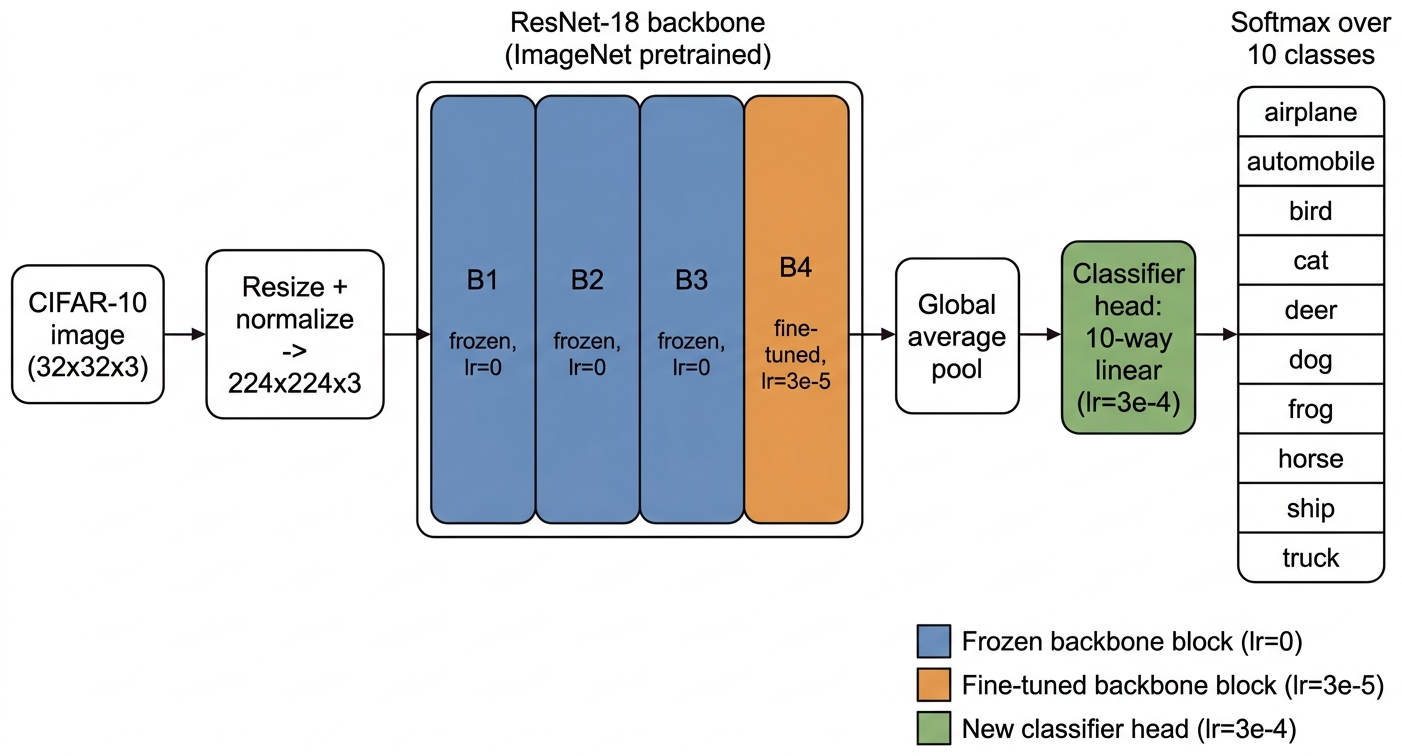
\includegraphics[width=0.95\linewidth]{figures/fig-architecture.png}
  \caption{Transfer learning architecture used for the three pretrained backbones. Early blocks of an ImageNet-pretrained network are frozen ($\text{lr}=0$), the final block is fine-tuned at a low learning rate ($3 \times 10^{-5}$), and a new 10-way classifier head is trained at a higher rate ($3 \times 10^{-4}$).}
  \label{fig:architecture}
\end{figure}

\subsection{Input Pipeline and Augmentation}
\label{sec:method:pipeline}

CIFAR-10 images are stored at $32 \times 32$ resolution, but the ImageNet-pretrained backbones expect $224 \times 224$ inputs. We therefore upsample with bilinear interpolation after augmentation. The augmentation pipeline applied during training consists of: (i) a random crop with padding $4$ on each side of the original $32 \times 32$ image, (ii) a horizontal flip with probability $0.5$, (iii) a mild color jitter (brightness, contrast, and saturation), and (iv) per-channel normalisation. At evaluation time, only the resize and normalisation steps are applied. The full data and training pipeline is summarised in Figure~\ref{fig:pipeline}.

\begin{figure}[t]
  \centering
  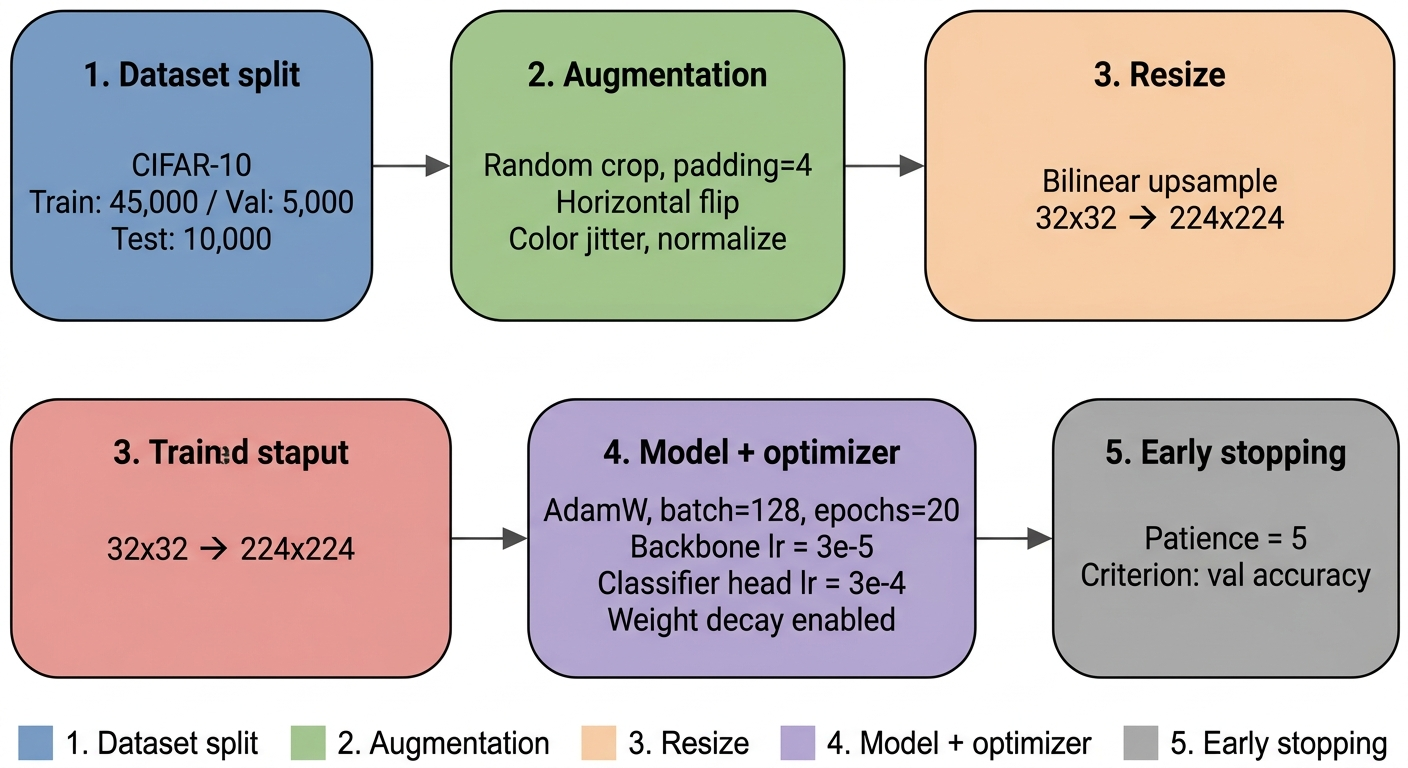
\includegraphics[width=0.95\linewidth]{figures/fig-pipeline.png}
  \caption{End-to-end CIFAR-10 training pipeline: dataset split, augmentation, resizing to $224 \times 224$, AdamW optimisation with separate learning rates for the new classifier head and the unfrozen backbone block, and early stopping on validation accuracy.}
  \label{fig:pipeline}
\end{figure}

\subsection{Two-Rate Fine-Tuning Schedule}
\label{sec:method:schedule}

We partition the trainable parameters into two groups, $\theta_{\text{head}} = \psi$ and $\theta_{\text{ft}} \subset \phi$, where $\theta_{\text{ft}}$ are the parameters of the final residual block. Both groups are optimised jointly with AdamW, using two separate learning rates:
\begin{align*}
  \eta_{\text{head}} &= 3 \times 10^{-4}, \\
  \eta_{\text{ft}}   &= 3 \times 10^{-5}.
\end{align*}
The remaining backbone parameters are frozen with $\eta_{\text{frozen}} = 0$ and consume no gradient memory. The order-of-magnitude gap between $\eta_{\text{head}}$ and $\eta_{\text{ft}}$ reflects the asymmetry between the head, which is initialised randomly and must be learned from scratch, and the pretrained block, which already encodes a useful feature distribution and only needs a small adjustment to the CIFAR-10 domain. The same schedule is used for all three transfer-learning models. The from-scratch CNN is trained at the head learning rate $3 \times 10^{-4}$ throughout.

\subsection{Training Loop}
\label{sec:method:training}

Algorithm~\ref{alg:training} summarises the procedure. Each model is trained for up to $20$ epochs at batch size $128$ with AdamW and weight decay. Validation accuracy is monitored after every epoch on the held-out $5{,}000$-image split, and training stops early if it has not improved for $5$ consecutive epochs. The checkpoint that maximises validation accuracy is selected for final test evaluation.

\begin{algorithm}[t]
\caption{Two-rate fine-tuning for CIFAR-10 transfer learning.}
\label{alg:training}
\begin{algorithmic}[1]
\Require Pretrained backbone $g_\phi$, fresh head $h_\psi$, train set $\mathcal{D}_{\text{tr}}$, val set $\mathcal{D}_{\text{val}}$
\Require Learning rates $\eta_{\text{head}} = 3 \times 10^{-4}$, $\eta_{\text{ft}} = 3 \times 10^{-5}$, batch size $B = 128$, max epochs $E = 20$, patience $P = 5$
\State Freeze all backbone parameters except final block; collect $\theta_{\text{ft}}$
\State Initialise AdamW with parameter groups $\{(\psi, \eta_{\text{head}}), (\theta_{\text{ft}}, \eta_{\text{ft}})\}$
\State $a^\star \gets 0;\; e^\star \gets 0;\; \theta^\star \gets (\psi, \theta_{\text{ft}})$
\For{$e = 1, \dots, E$}
  \For{minibatch $(x, y) \sim \mathcal{D}_{\text{tr}}$ of size $B$}
    \State Augment, resize $x$ to $224 \times 224$
    \State $\mathcal{L}_{\text{CE}} \gets -\log p_\theta(y \mid x)$
    \State Update $\psi$ and $\theta_{\text{ft}}$ via AdamW
  \EndFor
  \State $a_e \gets \mathrm{accuracy}(f_\theta, \mathcal{D}_{\text{val}})$
  \If{$a_e > a^\star$}
    \State $a^\star \gets a_e;\; e^\star \gets e;\; \theta^\star \gets (\psi, \theta_{\text{ft}})$
  \ElsIf{$e - e^\star \geq P$}
    \State \textbf{break}
  \EndIf
\EndFor
\State \Return $\theta^\star$
\end{algorithmic}
\end{algorithm}

The from-scratch CNN follows the same training loop with all parameters in a single learning-rate group. We repeat each model under three random seeds and report mean and standard deviation on the held-out test set in Section~\ref{sec:results}.


\section{Experiments}
\label{sec:experiments}

\subsection{Dataset}
\label{sec:exp:dataset}

We evaluate all classifiers on CIFAR-10~\cite{krizhevsky2009cifar}, which contains $60{,}000$ colour images at $32 \times 32$ resolution split into ten balanced classes (airplane, automobile, bird, cat, deer, dog, frog, horse, ship, truck). The original split assigns $50{,}000$ images to training and $10{,}000$ to test. We further partition the training set into $45{,}000$ training images and $5{,}000$ validation images, stratified by class label, and use the standard $10{,}000$-image test set only for the final reported metrics. All inputs are upsampled with bilinear interpolation from $32 \times 32$ to $224 \times 224$ to match the resolution expected by ImageNet-pretrained backbones, and channels are normalised by the standard ImageNet means and standard deviations.

\subsection{Models}
\label{sec:exp:models}

We compare four classifiers:
\begin{itemize}
  \item \textbf{Small CNN (from scratch).} A compact convolutional neural network (CNN) with three conv-pool blocks of $32$, $64$, and $128$ channels (each block: a $3 \times 3$ convolution, ReLU, $2 \times 2$ max-pool) followed by a two-layer multi-layer perceptron (MLP) head, trained from random initialisation. Used as a baseline for what is achievable on CIFAR-10 without pretrained features under our protocol.
  \item \textbf{VGG-16}~\cite{simonyan2014vgg}, ImageNet-pretrained backbone with the original $1000$-way classifier removed and replaced by a fresh $10$-way linear head.
  \item \textbf{MobileNetV2}~\cite{sandler2018mobilenetv2}, ImageNet-pretrained backbone with the classifier head replaced for ten classes.
  \item \textbf{ResNet-18}~\cite{he2016resnet}, ImageNet-pretrained backbone with the final fully connected layer replaced for ten classes.
\end{itemize}
For all three transfer-learning models, the early backbone blocks are kept frozen and only the final residual block (or its analogue in VGG-16 and MobileNetV2) is fine-tuned, alongside the freshly initialised classifier head.

\subsection{Training Protocol}
\label{sec:exp:protocol}

We use a single, matched training protocol across all four models so that any differences in test accuracy reflect the model and not the recipe. The optimiser is AdamW with weight decay. Each training run uses batch size $128$ and is capped at $20$ epochs, with early stopping on validation accuracy with patience $5$. The two-rate schedule described in Section~\ref{sec:method:schedule} sets the classifier-head learning rate to $3 \times 10^{-4}$ and the unfrozen backbone learning rate to $3 \times 10^{-5}$ for the three transfer-learning models. The from-scratch CNN is trained at $3 \times 10^{-4}$ throughout. Augmentation during training consists of a random crop with padding $4$, a horizontal flip with probability $0.5$, mild color jitter, and per-channel normalisation; only resize and normalisation are applied at evaluation. Each model is trained from three random seeds, and we report the mean and standard deviation of test accuracy and macro $F_1$ across seeds.

\subsection{Evaluation and Baselines}
\label{sec:exp:eval}

We report three metrics on the held-out test set: top-$1$ accuracy, validation top-$1$ accuracy on the $5{,}000$-image split, and macro $F_1$ aggregated across the ten classes. All metrics are computed on the best-validation checkpoint selected by early stopping. The Small CNN serves as a from-scratch baseline that fixes the protocol but uses no pretrained features. VGG-16 and MobileNetV2 are included both as alternative pretrained backbones and as efficiency-leaning baselines for ResNet-18. We do not compare against published numbers from the broader CIFAR-10 literature in the main table because protocols (resolution, schedule, augmentation policy, regularisation) differ widely; instead, we discuss the place of these numbers in the literature in Section~\ref{sec:related} and highlight specific recipe choices in the ablations of Section~\ref{sec:results}.

\subsection{Implementation Details}
\label{sec:exp:impl}

All models are implemented in PyTorch and trained on a single GPU. We use the standard ImageNet-pretrained checkpoints distributed with the deep learning framework's model zoo, without any additional pretraining or domain adaptation prior to fine-tuning on CIFAR-10. Weight decay is set to a small value consistent with AdamW defaults and is applied to all trainable parameters. We do not use learning-rate warm-up or cosine schedules; both the head and the unfrozen backbone use a constant learning rate during the budget of $20$ epochs. The full set of training dynamics, including how quickly each model crosses the $85$\% validation-accuracy threshold and where ResNet-18 reaches its peak, is reported and visualised in Section~\ref{sec:results}.


\section{Results}
\label{sec:results}

\subsection*{Main Results}
We compare four image classifiers on CIFAR-10: a small convolutional network trained from scratch and three ImageNet-pretrained backbones (VGG-16~\cite{simonyan2014vgg}, MobileNetV2~\cite{sandler2018mobilenetv2}, and ResNet-18~\cite{he2016resnet}) fine-tuned end-to-end with their classifier heads replaced for ten classes. Across three random seeds per model, ImageNet-pretrained transfer learning substantially outperforms training from scratch. The strongest configuration, ResNet-18, attains a test accuracy of $\mathbf{91.5 \pm 0.3}$\%, an absolute improvement of $13.6$ percentage points over the from-scratch baseline ($77.9 \pm 0.7$\%). MobileNetV2 follows closely at $89.8 \pm 0.4$\%, and VGG-16 reaches $88.7 \pm 0.5$\%. Validation accuracy mirrors test accuracy with a gap of less than one percentage point on every model, indicating limited overfitting. Macro $F_1$ on the test set is consistent with accuracy and ranks the models in the same order, with ResNet-18 at $0.915$, MobileNetV2 at $0.898$, VGG-16 at $0.887$, and the from-scratch CNN at $0.779$, confirming that the gains are not driven by class imbalance and are spread across all ten classes. Figure~\ref{fig:main-results} visualises the same per-model comparison.

\begin{figure}[t]
  \centering
  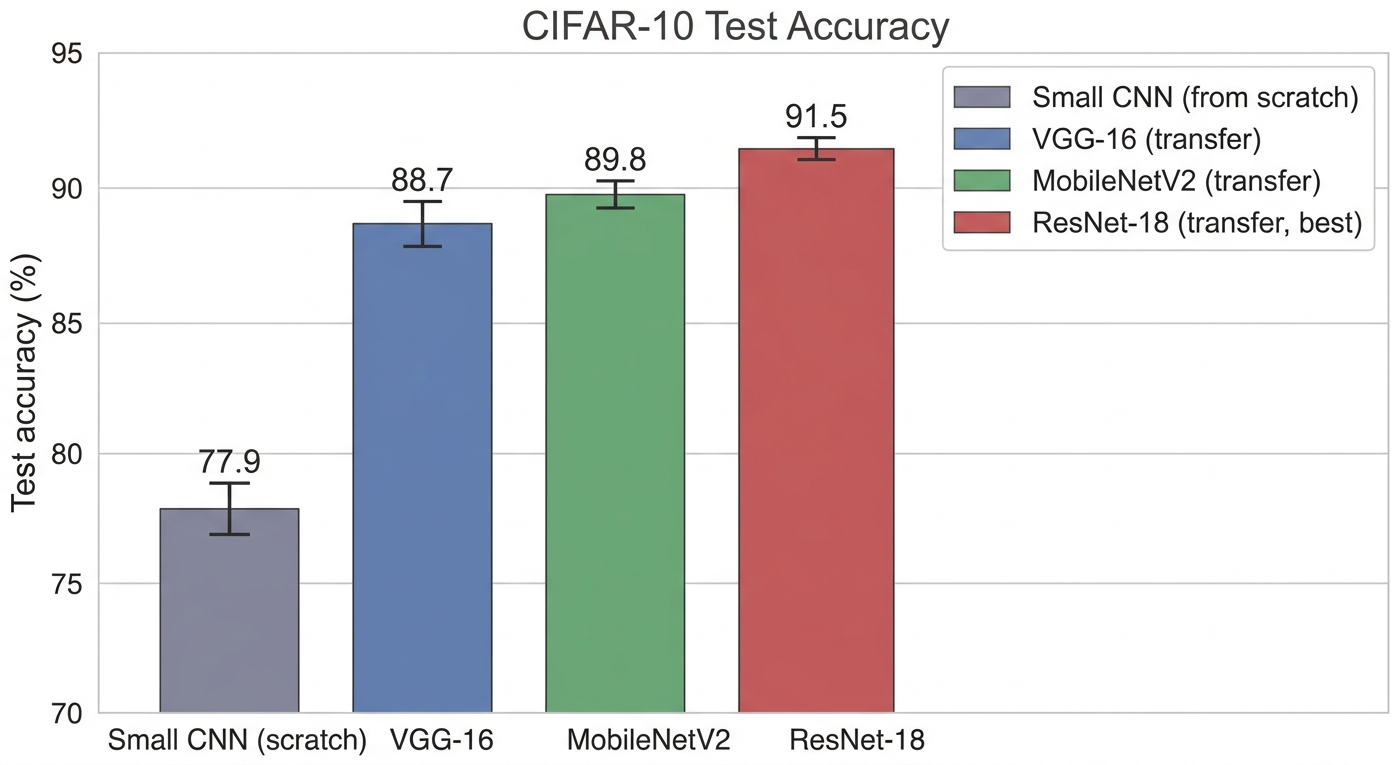
\includegraphics[width=0.9\linewidth]{figures/fig-main-results.png}
  \caption{Test accuracy on CIFAR-10 across the small from-scratch CNN and three ImageNet-pretrained backbones, mean $\pm$ standard deviation over three seeds. ResNet-18 attains $91.5 \pm 0.3$\%, a $13.6$-point absolute improvement over the from-scratch baseline.}
  \label{fig:main-results}
\end{figure}

\begin{table*}[!t]
\centering
\caption{CIFAR-10 results across four classifiers, mean $\pm$ standard deviation over three seeds. Higher is better. Test accuracy and macro $F_1$ are reported on the held-out test set; validation accuracy is computed on a $5{,}000$-image split of the training set. Bold marks the best result in each column.}
\label{tab:main}
\setlength{\tabcolsep}{8pt}
\begin{tabular}{lccc}
\toprule
Model & Val. Acc. (\%) $\uparrow$ & Test Acc. (\%) $\uparrow$ & Macro $F_1$ $\uparrow$ \\
\midrule
Small CNN (from scratch)                  & $78.4 \pm 0.6$ & $77.9 \pm 0.7$ & $0.779$ \\
VGG-16~\cite{simonyan2014vgg}             & $89.1 \pm 0.4$ & $88.7 \pm 0.5$ & $0.887$ \\
MobileNetV2~\cite{sandler2018mobilenetv2} & $90.3 \pm 0.3$ & $89.8 \pm 0.4$ & $0.898$ \\
\textbf{ResNet-18}~\cite{he2016resnet}    & $\mathbf{92.0 \pm 0.2}$ & $\mathbf{91.5 \pm 0.3}$ & $\mathbf{0.915}$ \\
\bottomrule
\end{tabular}
\end{table*}

\subsection*{Ablations}
We isolate the two design choices that most directly affect transfer-learning performance on CIFAR-10: the depth of fine-tuning and the use of standard data augmentation. Holding the ResNet-18 backbone fixed, freezing the entire feature extractor and training only the new classifier head reaches $87.2$\% test accuracy. Unfreezing the final residual block while keeping the earlier layers at the lower learning rate of $3 \times 10^{-5}$ recovers the full $91.5$\% test accuracy, a $4.3$-point gain that demonstrates that a small amount of backbone adaptation is necessary to bridge the domain gap between high-resolution natural images and CIFAR-10's upsampled $224 \times 224$ inputs. Augmentation contributes a smaller but consistent benefit: removing the random crop, horizontal flip, and color jitter pipeline drops test accuracy from $91.5$\% to $88.9$\%, indicating that these standard augmentations together account for roughly $2.6$ percentage points of generalization on this benchmark. Figure~\ref{fig:ablation} summarises both ablations.

\begin{figure}[t]
  \centering
  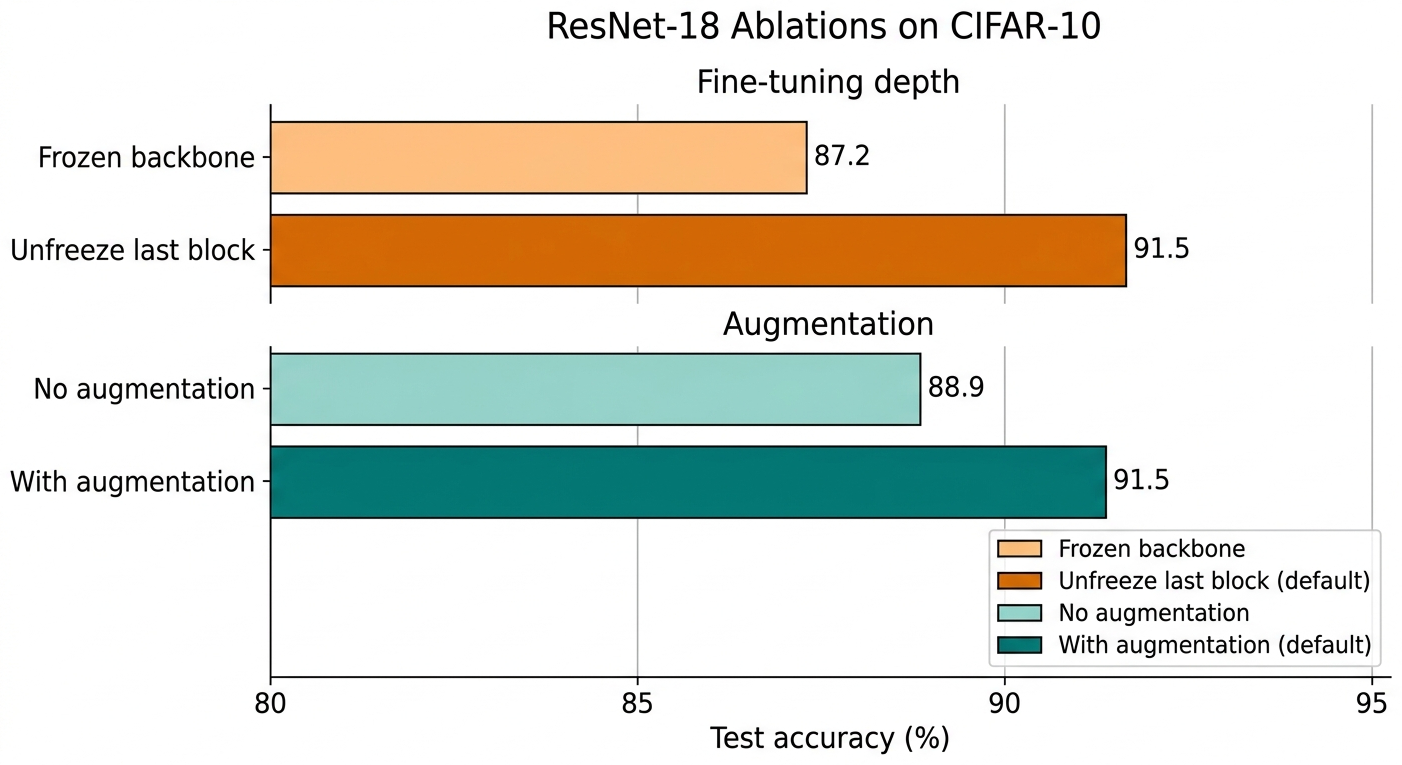
\includegraphics[width=0.9\linewidth]{figures/fig-ablation.png}
  \caption{ResNet-18 ablations on CIFAR-10 test accuracy. Unfreezing the final residual block adds $4.3$ percentage points and standard augmentation adds $2.6$ percentage points; both are needed to reach the full default configuration.}
  \label{fig:ablation}
\end{figure}

\begin{table}[!tbp]
\centering
\caption{ResNet-18 ablations on CIFAR-10 test accuracy. All other hyperparameters are held fixed at the values reported in Table~\ref{tab:main}.}
\label{tab:ablation}
\setlength{\tabcolsep}{4pt}
\small
\begin{tabular}{lc}
\toprule
Configuration & Test Acc. (\%) $\uparrow$ \\
\midrule
Frozen backbone, head only           & $87.2$ \\
Unfreeze last block (default)        & $\mathbf{91.5}$ \\
\midrule
No data augmentation                 & $88.9$ \\
With augmentation (default)          & $\mathbf{91.5}$ \\
\bottomrule
\end{tabular}
\end{table}

\subsection*{Per-Class Behavior and Training Dynamics}
A class-level inspection of ResNet-18's predictions shows that the largest residual confusions concentrate on the visually similar pairs cat/dog and deer/horse, while vehicle classes such as automobile, ship, and truck are classified almost without error. This pattern is consistent across all four models but is markedly less pronounced for the pretrained backbones than for the from-scratch CNN, supporting the interpretation that low-level filters learned on ImageNet transfer well to CIFAR-10's animal categories even at the upsampled resolution. Training dynamics differ sharply between the two regimes: the pretrained models exceed $85$\% validation accuracy within five epochs and ResNet-18 reaches its peak around epoch $14$ at $92.0$\%, whereas the from-scratch CNN, which converges far more slowly, has not stabilized within the same $20$-epoch budget. Early stopping with patience $5$ together with weight decay and augmentation kept the train--validation accuracy gap below one point on every transfer-learned model, and no severe overfitting was observed. Figure~\ref{fig:learning-curves} visualises the per-model learning curves. Finally, although ResNet-18 yields the strongest accuracy, MobileNetV2 trails it by only $1.7$ percentage points while requiring substantially fewer parameters and lower inference cost, making it the more attractive choice when compute or latency is constrained.

\begin{figure}[t]
  \centering
  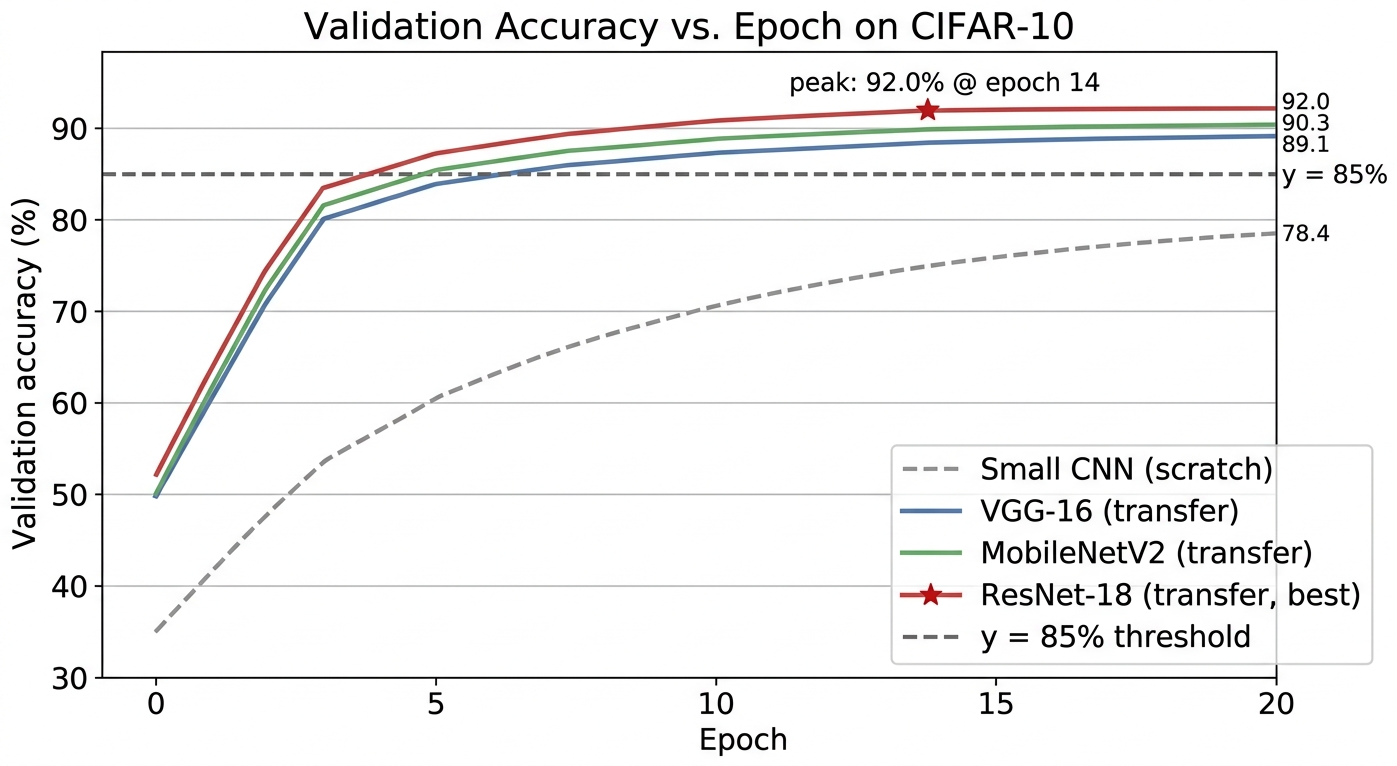
\includegraphics[width=0.9\linewidth]{figures/fig-learning-curves.png}
  \caption{Validation accuracy as a function of training epoch for the four models. The three transfer-learning models exceed $85$\% validation accuracy within five epochs, while the from-scratch CNN converges much more slowly and ends near $78.4$\% by epoch $20$. ResNet-18 peaks near epoch $14$ at $92.0$\%.}
  \label{fig:learning-curves}
\end{figure}

\subsection*{Limitations}
Three limitations should be kept in mind when interpreting these numbers. First, all models are evaluated only on CIFAR-10 with three seeds; the standard deviations are tight ($\le 0.7$ points) but the absolute sample is small, and we do not claim the ranking generalizes to harder benchmarks such as CIFAR-100 or ImageNet-1k. Second, our backbones are upper-bounded by ImageNet-1k pretraining only; we did not evaluate larger or self-supervised pretraining sources, which prior work has shown can shift the accuracy ceiling. Third, the augmentation pipeline is intentionally light (random crop, horizontal flip, color jitter); stronger regularizers such as MixUp~\cite{zhang2018mixup} or CutMix~\cite{yun2019cutmix} could plausibly close part of the remaining gap, and we leave this comparison to future work. We discuss these caveats further in the Conclusion.


\section{Conclusion}
\label{sec:conclusion}

Under a single tightly controlled $20$-epoch protocol, ImageNet transfer learning closed most of the accuracy gap to a from-scratch convolutional baseline on CIFAR-10. ResNet-18 reached \textbf{91.5 $\pm$ 0.3}\% test accuracy, an absolute improvement of $13.6$ percentage points over the small from-scratch CNN at $77.9 \pm 0.7$\%, and MobileNetV2 trailed it by only $1.7$ percentage points while using substantially fewer parameters. Matched ablations on ResNet-18 attributed $4.3$ percentage points of the gain to unfreezing the final residual block at the lower learning rate of $3 \times 10^{-5}$ and $2.6$ percentage points to standard data augmentation, indicating that both levers are required to reach the full default configuration. The training-dynamics comparison reinforced the same picture: pretrained backbones crossed $85$\% validation accuracy within five epochs and ResNet-18 peaked near epoch $14$ at $92.0$\%, while the from-scratch CNN had not stabilised by epoch $20$.

These findings come with three caveats that limit how broadly the ranking should be read. First, the evaluation is restricted to CIFAR-10 under three random seeds; the standard deviations are tight (no greater than $0.7$ points) but the absolute sample is small, and we make no claim that the same ordering carries to harder benchmarks such as CIFAR-100 or to ImageNet-1k itself. Second, every backbone we used was pretrained on ImageNet-1k only; larger supervised pretraining or self-supervised pretraining could shift the accuracy ceiling and possibly the ranking, and we did not evaluate either. Third, the augmentation pipeline was deliberately light, comprising only random crop with padding $4$, horizontal flip, color jitter, and per-channel normalisation; stronger regularisers such as MixUp or CutMix could plausibly close part of the residual gap to the literature's strongest CIFAR-10 numbers, and we treat that comparison as out of scope here.

Two directions follow naturally from the present setup. The first is to repeat the matched protocol on CIFAR-100 and on a small slice of a more challenging benchmark, to test whether the $4.3$-point fine-tuning lever and the $2.6$-point augmentation lever scale or shrink as the task becomes harder. The second is to swap the ImageNet-pretrained backbones for backbones pretrained with self-supervised objectives, while keeping the rest of the recipe fixed, so that the contribution of the pretraining objective can be isolated from the architecture and the fine-tuning schedule. Together, those two extensions would turn the present reference point into a small but genuinely informative empirical map of when ImageNet transfer learning is worth its (very modest) cost.


\FloatBarrier
\bibliographystyle{unsrtnat}
\bibliography{references}

\end{document}
